% Options for packages loaded elsewhere
\PassOptionsToPackage{unicode}{hyperref}
\PassOptionsToPackage{hyphens}{url}
%
\documentclass[
]{article}
\usepackage{amsmath,amssymb}
\usepackage{iftex}
\ifPDFTeX
  \usepackage[T1]{fontenc}
  \usepackage[utf8]{inputenc}
  \usepackage{textcomp} % provide euro and other symbols
\else % if luatex or xetex
  \usepackage{unicode-math} % this also loads fontspec
  \defaultfontfeatures{Scale=MatchLowercase}
  \defaultfontfeatures[\rmfamily]{Ligatures=TeX,Scale=1}
\fi
\usepackage{lmodern}
\ifPDFTeX\else
  % xetex/luatex font selection
\fi
% Use upquote if available, for straight quotes in verbatim environments
\IfFileExists{upquote.sty}{\usepackage{upquote}}{}
\IfFileExists{microtype.sty}{% use microtype if available
  \usepackage[]{microtype}
  \UseMicrotypeSet[protrusion]{basicmath} % disable protrusion for tt fonts
}{}
\makeatletter
\@ifundefined{KOMAClassName}{% if non-KOMA class
  \IfFileExists{parskip.sty}{%
    \usepackage{parskip}
  }{% else
    \setlength{\parindent}{0pt}
    \setlength{\parskip}{6pt plus 2pt minus 1pt}}
}{% if KOMA class
  \KOMAoptions{parskip=half}}
\makeatother
\usepackage{xcolor}
\usepackage[margin=1in]{geometry}
\usepackage{color}
\usepackage{fancyvrb}
\newcommand{\VerbBar}{|}
\newcommand{\VERB}{\Verb[commandchars=\\\{\}]}
\DefineVerbatimEnvironment{Highlighting}{Verbatim}{commandchars=\\\{\}}
% Add ',fontsize=\small' for more characters per line
\usepackage{framed}
\definecolor{shadecolor}{RGB}{248,248,248}
\newenvironment{Shaded}{\begin{snugshade}}{\end{snugshade}}
\newcommand{\AlertTok}[1]{\textcolor[rgb]{0.94,0.16,0.16}{#1}}
\newcommand{\AnnotationTok}[1]{\textcolor[rgb]{0.56,0.35,0.01}{\textbf{\textit{#1}}}}
\newcommand{\AttributeTok}[1]{\textcolor[rgb]{0.13,0.29,0.53}{#1}}
\newcommand{\BaseNTok}[1]{\textcolor[rgb]{0.00,0.00,0.81}{#1}}
\newcommand{\BuiltInTok}[1]{#1}
\newcommand{\CharTok}[1]{\textcolor[rgb]{0.31,0.60,0.02}{#1}}
\newcommand{\CommentTok}[1]{\textcolor[rgb]{0.56,0.35,0.01}{\textit{#1}}}
\newcommand{\CommentVarTok}[1]{\textcolor[rgb]{0.56,0.35,0.01}{\textbf{\textit{#1}}}}
\newcommand{\ConstantTok}[1]{\textcolor[rgb]{0.56,0.35,0.01}{#1}}
\newcommand{\ControlFlowTok}[1]{\textcolor[rgb]{0.13,0.29,0.53}{\textbf{#1}}}
\newcommand{\DataTypeTok}[1]{\textcolor[rgb]{0.13,0.29,0.53}{#1}}
\newcommand{\DecValTok}[1]{\textcolor[rgb]{0.00,0.00,0.81}{#1}}
\newcommand{\DocumentationTok}[1]{\textcolor[rgb]{0.56,0.35,0.01}{\textbf{\textit{#1}}}}
\newcommand{\ErrorTok}[1]{\textcolor[rgb]{0.64,0.00,0.00}{\textbf{#1}}}
\newcommand{\ExtensionTok}[1]{#1}
\newcommand{\FloatTok}[1]{\textcolor[rgb]{0.00,0.00,0.81}{#1}}
\newcommand{\FunctionTok}[1]{\textcolor[rgb]{0.13,0.29,0.53}{\textbf{#1}}}
\newcommand{\ImportTok}[1]{#1}
\newcommand{\InformationTok}[1]{\textcolor[rgb]{0.56,0.35,0.01}{\textbf{\textit{#1}}}}
\newcommand{\KeywordTok}[1]{\textcolor[rgb]{0.13,0.29,0.53}{\textbf{#1}}}
\newcommand{\NormalTok}[1]{#1}
\newcommand{\OperatorTok}[1]{\textcolor[rgb]{0.81,0.36,0.00}{\textbf{#1}}}
\newcommand{\OtherTok}[1]{\textcolor[rgb]{0.56,0.35,0.01}{#1}}
\newcommand{\PreprocessorTok}[1]{\textcolor[rgb]{0.56,0.35,0.01}{\textit{#1}}}
\newcommand{\RegionMarkerTok}[1]{#1}
\newcommand{\SpecialCharTok}[1]{\textcolor[rgb]{0.81,0.36,0.00}{\textbf{#1}}}
\newcommand{\SpecialStringTok}[1]{\textcolor[rgb]{0.31,0.60,0.02}{#1}}
\newcommand{\StringTok}[1]{\textcolor[rgb]{0.31,0.60,0.02}{#1}}
\newcommand{\VariableTok}[1]{\textcolor[rgb]{0.00,0.00,0.00}{#1}}
\newcommand{\VerbatimStringTok}[1]{\textcolor[rgb]{0.31,0.60,0.02}{#1}}
\newcommand{\WarningTok}[1]{\textcolor[rgb]{0.56,0.35,0.01}{\textbf{\textit{#1}}}}
\usepackage{graphicx}
\makeatletter
\def\maxwidth{\ifdim\Gin@nat@width>\linewidth\linewidth\else\Gin@nat@width\fi}
\def\maxheight{\ifdim\Gin@nat@height>\textheight\textheight\else\Gin@nat@height\fi}
\makeatother
% Scale images if necessary, so that they will not overflow the page
% margins by default, and it is still possible to overwrite the defaults
% using explicit options in \includegraphics[width, height, ...]{}
\setkeys{Gin}{width=\maxwidth,height=\maxheight,keepaspectratio}
% Set default figure placement to htbp
\makeatletter
\def\fps@figure{htbp}
\makeatother
\setlength{\emergencystretch}{3em} % prevent overfull lines
\providecommand{\tightlist}{%
  \setlength{\itemsep}{0pt}\setlength{\parskip}{0pt}}
\setcounter{secnumdepth}{-\maxdimen} % remove section numbering
\ifLuaTeX
  \usepackage{selnolig}  % disable illegal ligatures
\fi
\usepackage{bookmark}
\IfFileExists{xurl.sty}{\usepackage{xurl}}{} % add URL line breaks if available
\urlstyle{same}
\hypersetup{
  pdftitle={Introduction to R and RStudio},
  hidelinks,
  pdfcreator={LaTeX via pandoc}}

\title{Introduction to R and RStudio}
\author{}
\date{\vspace{-2.5em}2024-05-01}

\begin{document}
\maketitle

\phantomsection\label{instructions}
Complete all \textbf{Exercises}, and submit answers to
\textbf{Questions} on the Coursera platform.

The goal of this lab is to introduce you to R and RStudio, which you'll
be using throughout the course both to learn the statistical concepts
discussed in the course and to analyze real data and come to informed
conclusions. To straighten out which is which: R is the name of the
programming language itself and RStudio is a convenient interface.

As the labs progress, you are encouraged to explore beyond what the labs
dictate; a willingness to experiment will make you a much better
programmer. Before we get to that stage, however, you need to build some
basic fluency in R. Today we begin with the fundamental building blocks
of R and RStudio: the interface, reading in data, and basic commands.

\subsection{RStudio}\label{rstudio}

Your RStudio window has four panels.

Your R Markdown file (this document) is in the upper left panel.

The panel on the lower left is where the action happens. It's called the
\emph{console}. Everytime you launch RStudio, it will have the same text
at the top of the console telling you the version of R that you're
running. Below that information is the \emph{prompt}. As its name
suggests, this prompt is really a request, a request for a command.
Initially, interacting with R is all about typing commands and
interpreting the output. These commands and their syntax have evolved
over decades (literally) and now provide what many users feel is a
fairly natural way to access data and organize, describe, and invoke
statistical computations.

The panel in the upper right contains your \emph{workspace} as well as a
history of the commands that you've previously entered.

Any plots that you generate will show up in the panel in the lower right
corner. This is also where you can browse your files, access help,
manage packages, etc.

\subsection{R Packages}\label{r-packages}

R is an open-source programming language, meaning that users can
contribute packages that make our lives easier, and we can use them for
free. For this lab, and many others in the future, we will use the
following R packages:

\begin{itemize}
\tightlist
\item
  \texttt{statsr}: for data files and functions used in this course
\item
  \texttt{dplyr}: for data wrangling
\item
  \texttt{ggplot2}: for data visualization
\end{itemize}

You should have already installed these packages using commands like
\texttt{install.packages} and \texttt{install\_github}.

Next, you need to load the packages in your working environment. We do
this with the \texttt{library} function. Note that you only need to
\textbf{install} packages once, but you need to \textbf{load} them each
time you relaunch RStudio.

\begin{Shaded}
\begin{Highlighting}[]
\FunctionTok{library}\NormalTok{(dplyr)}
\FunctionTok{library}\NormalTok{(ggplot2)}
\FunctionTok{library}\NormalTok{(statsr)}
\end{Highlighting}
\end{Shaded}

To do so, you can

\begin{itemize}
\tightlist
\item
  click on the green arrow at the top of the code chunk in the R
  Markdown (Rmd) file, or
\item
  highlight these lines, and hit the \textbf{Run} button on the upper
  right corner of the pane, or
\item
  type the code in the console.
\end{itemize}

Going forward you will be asked to load any relevant packages at the
beginning of each lab.

\subsection{Dataset 1: Dr.~Arbuthnot's Baptism
Records}\label{dataset-1-dr.-arbuthnots-baptism-records}

To get you started, run the following command to load the data.

\begin{Shaded}
\begin{Highlighting}[]
\FunctionTok{data}\NormalTok{(arbuthnot)}
\end{Highlighting}
\end{Shaded}

To do so, once again, you can

\begin{itemize}
\tightlist
\item
  click on the green arrow at the top of the code chunk in the R
  Markdown (Rmd) file, or
\item
  put your cursor on this line, and hit the \textbf{Run} button on the
  upper right corner of the pane, or
\item
  type the code in the console.
\end{itemize}

This command instructs R to load some data. The Arbuthnot baptism counts
for boys and girls. You should see that the workspace area in the upper
righthand corner of the RStudio window now lists a data set called
\texttt{arbuthnot} that has 82 observations on 3 variables. As you
interact with R, you will create a series of objects. Sometimes you load
them as we have done here, and sometimes you create them yourself as the
byproduct of a computation or some analysis you have performed.

The Arbuthnot data set refers to Dr.~John Arbuthnot, an 18th century
physician, writer, and mathematician. He was interested in the ratio of
newborn boys to newborn girls, so he gathered the baptism records for
children born in London for every year from 1629 to 1710. We can take a
look at the data by typing its name into the console.

\begin{Shaded}
\begin{Highlighting}[]
\NormalTok{arbuthnot}
\end{Highlighting}
\end{Shaded}

\begin{verbatim}
## # A tibble: 82 x 3
##     year  boys girls
##    <int> <int> <int>
##  1  1629  5218  4683
##  2  1630  4858  4457
##  3  1631  4422  4102
##  4  1632  4994  4590
##  5  1633  5158  4839
##  6  1634  5035  4820
##  7  1635  5106  4928
##  8  1636  4917  4605
##  9  1637  4703  4457
## 10  1638  5359  4952
## # i 72 more rows
\end{verbatim}

However printing the whole dataset in the console is not that useful.
One advantage of RStudio is that it comes with a built-in data viewer.
Click on the name \texttt{arbuthnot} in the \emph{Environment} pane
(upper right window) that lists the objects in your workspace. This will
bring up an alternative display of the data set in the \emph{Data
Viewer} (upper left window). You can close the data viewer by clicking
on the \emph{x} in the upper lefthand corner.

What you should see are four columns of numbers, each row representing a
different year: the first entry in each row is simply the row number (an
index we can use to access the data from individual years if we want),
the second is the year, and the third and fourth are the numbers of boys
and girls baptized that year, respectively. Use the scrollbar on the
right side of the console window to examine the complete data set.

Note that the row numbers in the first column are not part of
Arbuthnot's data. R adds them as part of its printout to help you make
visual comparisons. You can think of them as the index that you see on
the left side of a spreadsheet. In fact, the comparison to a spreadsheet
will generally be helpful. R has stored Arbuthnot's data in a kind of
spreadsheet or table called a \emph{data frame}.

You can see the dimensions of this data frame by typing:

\begin{Shaded}
\begin{Highlighting}[]
\FunctionTok{dim}\NormalTok{(arbuthnot)}
\end{Highlighting}
\end{Shaded}

\begin{verbatim}
## [1] 82  3
\end{verbatim}

This command should output \texttt{{[}1{]}\ 82\ 3}, indicating that
there are 82 rows and 3 columns (we'll get to what the \texttt{{[}1{]}}
means in a bit), just as it says next to the object in your workspace.
You can see the names of these columns (or variables) by typing:

\begin{Shaded}
\begin{Highlighting}[]
\FunctionTok{names}\NormalTok{(arbuthnot)}
\end{Highlighting}
\end{Shaded}

\begin{verbatim}
## [1] "year"  "boys"  "girls"
\end{verbatim}

\begin{enumerate}
\def\labelenumi{\arabic{enumi}.}
\tightlist
\item
  How many variables are included in this data set?

  2

  3

  4

  82

  1710
\end{enumerate}

\phantomsection\label{exercise}
\textbf{Exercise}: What years are included in this dataset? Hint: Take a
look at the year variable in the Data Viewer to answer this question.

You should see that the data frame contains the columns \texttt{year},
\texttt{boys}, and \texttt{girls}. At this point, you might notice that
many of the commands in R look a lot like functions from math class;
that is, invoking R commands means supplying a function with some number
of arguments. The \texttt{dim} and \texttt{names} commands, for example,
each took a single argument, the name of a data frame.

\phantomsection\label{boxedtext}
\textbf{Tip: } If you use the up and down arrow keys, you can scroll
through your previous commands, your so-called command history. You can
also access it by clicking on the history tab in the upper right panel.
This will save you a lot of typing in the future.

\subsubsection{R Markdown}\label{r-markdown}

So far we asked you to type your commands in the console. The console is
a great place for playing around with some code, however it is not a
good place for documenting your work. Working in the console exclusively
makes it difficult to document your work as you go, and reproduce it
later.

R Markdown is a great solution for this problem. And, you already have
worked with an R Markdown document -- this lab! Going forward type the
code for the questions in the code chunks provided in the R Markdown
(Rmd) document for the lab, and \textbf{Knit} the document to see the
results.

\subsubsection{Some Exploration}\label{some-exploration}

Let's start to examine the data a little more closely. We can access the
data in a single column of a data frame separately using a command like

\begin{Shaded}
\begin{Highlighting}[]
\NormalTok{arbuthnot}\SpecialCharTok{$}\NormalTok{boys}
\end{Highlighting}
\end{Shaded}

\begin{verbatim}
##  [1] 5218 4858 4422 4994 5158 5035 5106 4917 4703 5359 5366 5518 5470 5460 4793
## [16] 4107 4047 3768 3796 3363 3079 2890 3231 3220 3196 3441 3655 3668 3396 3157
## [31] 3209 3724 4748 5216 5411 6041 5114 4678 5616 6073 6506 6278 6449 6443 6073
## [46] 6113 6058 6552 6423 6568 6247 6548 6822 6909 7577 7575 7484 7575 7737 7487
## [61] 7604 7909 7662 7602 7676 6985 7263 7632 8062 8426 7911 7578 8102 8031 7765
## [76] 6113 8366 7952 8379 8239 7840 7640
\end{verbatim}

This command will only show the number of boys baptized each year. The
dollar sign basically says ``go to the data frame that comes before me,
and find the variable that comes after me''.

\begin{enumerate}
\def\labelenumi{\arabic{enumi}.}
\setcounter{enumi}{1}
\tightlist
\item
  What command would you use to extract just the counts of girls born?

  \texttt{arbuthnot\$boys}

  \texttt{arbuthnot\$girls}

  \texttt{girls}

  \texttt{arbuthnot{[}girls{]}}

  \texttt{\$girls}
\end{enumerate}

\begin{Shaded}
\begin{Highlighting}[]
\CommentTok{\# type your code for the Question 2 here, and Knit}
\NormalTok{arbuthnot}\SpecialCharTok{$}\NormalTok{girls}
\end{Highlighting}
\end{Shaded}

\begin{verbatim}
##  [1] 4683 4457 4102 4590 4839 4820 4928 4605 4457 4952 4784 5332 5200 4910 4617
## [16] 3997 3919 3395 3536 3181 2746 2722 2840 2908 2959 3179 3349 3382 3289 3013
## [31] 2781 3247 4107 4803 4881 5681 4858 4319 5322 5560 5829 5719 6061 6120 5822
## [46] 5738 5717 5847 6203 6033 6041 6299 6533 6744 7158 7127 7246 7119 7214 7101
## [61] 7167 7302 7392 7316 7483 6647 6713 7229 7767 7626 7452 7061 7514 7656 7683
## [76] 5738 7779 7417 7687 7623 7380 7288
\end{verbatim}

Notice that the way R has printed these data is different. When we
looked at the complete data frame, we saw 82 rows, one on each line of
the display. These data are no longer structured in a table with other
variables, so they are displayed one right after another. Objects that
print out in this way are called vectors; they represent a set of
numbers. R has added numbers in {[}brackets{]} along the left side of
the printout to indicate locations within the vector. For example, in
the arbuthnot\$boys vector, 5218 follows {[}1{]}, indicating that 5218
is the first entry in the vector. And if {[}43{]} starts a line, then
that would mean the first number on that line would represent the 43rd
entry in the vector.

R has some powerful functions for making graphics. We can create a
simple plot of the number of girls baptized per year with the command

\begin{Shaded}
\begin{Highlighting}[]
\FunctionTok{ggplot}\NormalTok{(}\AttributeTok{data =}\NormalTok{ arbuthnot, }\FunctionTok{aes}\NormalTok{(}\AttributeTok{x =}\NormalTok{ year, }\AttributeTok{y =}\NormalTok{ girls)) }\SpecialCharTok{+}
  \FunctionTok{geom\_point}\NormalTok{()}
\end{Highlighting}
\end{Shaded}

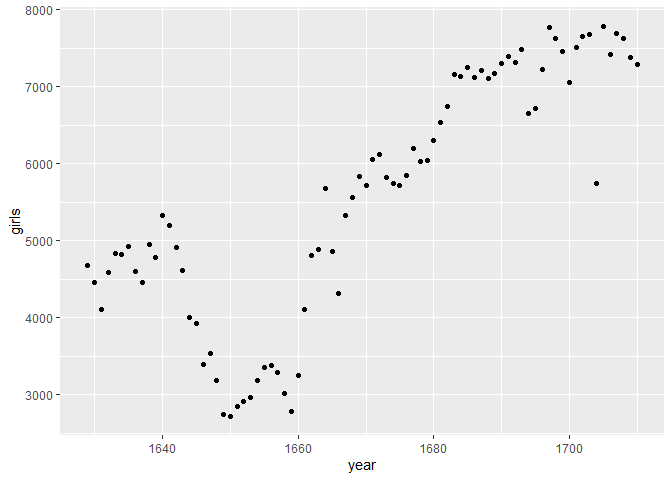
\includegraphics{lab_1_files/figure-latex/plot-girls-vs-year-1.pdf}

Before we review the code for this plot, let's summarize the trends we
see in the data.

\begin{enumerate}
\def\labelenumi{\arabic{enumi}.}
\tightlist
\item
  Which of the following best describes the number of girls baptised
  over the years included in this dataset?

  There appears to be no trend in the number of girls baptised from 1629
  to 1710.

  There is initially an increase in the number of girls baptised, which
  peaks around 1640. After 1640 there is a decrease in the number of
  girls baptised, but the number begins to increase again in 1660.
  Overall the trend is an increase in the number of girls baptised.

  There is initially an increase in the number of girls baptised. This
  number peaks around 1640 and then after 1640 the number of girls
  baptised decreases.

  The number of girls baptised has decreased over time.

  There is an initial increase in the number of girls baptised but this
  number appears to level around 1680 and not change after that time
  point.
\end{enumerate}

Back to the code\ldots{} We use the \texttt{ggplot()} function to build
plots. If you run the plotting code in your console, you should see the
plot appear under the \emph{Plots} tab of the lower right panel of
RStudio. Notice that the command above again looks like a function, this
time with arguments separated by commas.

\begin{itemize}
\tightlist
\item
  The first argument is always the dataset.
\item
  Next, we provide thevariables from the dataset to be assigned to
  \texttt{aes}thetic elements of the plot, e.g.~the x and the y axes.
\item
  Finally, we use another layer, separated by a \texttt{+} to specify
  the \texttt{geom}etric object for the plot. Since we want to
  scatterplot, we use \texttt{geom\_point}.
\end{itemize}

You might wonder how you are supposed to know the syntax for the
\texttt{ggplot} function. Thankfully, R documents all of its functions
extensively. To read what a function does and learn the arguments that
are available to you, just type in a question mark followed by the name
of the function that you're interested in. Try the following in your
console:

\begin{Shaded}
\begin{Highlighting}[]
\NormalTok{?ggplot}
\end{Highlighting}
\end{Shaded}

\begin{verbatim}
## starting httpd help server ... done
\end{verbatim}

Notice that the help file replaces the plot in the lower right panel.
You can toggle between plots and help files using the tabs at the top of
that panel.

\phantomsection\label{boxedtext}
More extensive help for plotting with the \texttt{ggplot2} package can
be found at \url{http://docs.ggplot2.org/current/}. The best (and
easiest) way to learn the syntax is to take a look at the sample plots
provided on that page, and modify the code bit by bit until you get
achieve the plot you want.

\subsubsection{R as a big calculator}\label{r-as-a-big-calculator}

Now, suppose we want to plot the total number of baptisms. To compute
this, we could use the fact that R is really just a big calculator. We
can type in mathematical expressions like

\begin{Shaded}
\begin{Highlighting}[]
\DecValTok{5218} \SpecialCharTok{+} \DecValTok{4683}
\end{Highlighting}
\end{Shaded}

\begin{verbatim}
## [1] 9901
\end{verbatim}

to see the total number of baptisms in 1629. We could repeat this once
for each year, but there is a faster way. If we add the vector for
baptisms for boys to that of girls, R will compute all sums
simultaneously.

\begin{Shaded}
\begin{Highlighting}[]
\NormalTok{arbuthnot}\SpecialCharTok{$}\NormalTok{boys }\SpecialCharTok{+}\NormalTok{ arbuthnot}\SpecialCharTok{$}\NormalTok{girls}
\end{Highlighting}
\end{Shaded}

\begin{verbatim}
##  [1]  9901  9315  8524  9584  9997  9855 10034  9522  9160 10311 10150 10850
## [13] 10670 10370  9410  8104  7966  7163  7332  6544  5825  5612  6071  6128
## [25]  6155  6620  7004  7050  6685  6170  5990  6971  8855 10019 10292 11722
## [37]  9972  8997 10938 11633 12335 11997 12510 12563 11895 11851 11775 12399
## [49] 12626 12601 12288 12847 13355 13653 14735 14702 14730 14694 14951 14588
## [61] 14771 15211 15054 14918 15159 13632 13976 14861 15829 16052 15363 14639
## [73] 15616 15687 15448 11851 16145 15369 16066 15862 15220 14928
\end{verbatim}

What you will see are 82 numbers (in that packed display, because we
aren’t looking at a data frame here), each one representing the sum
we’re after. Take a look at a few of them and verify that they are
right.

\subsubsection{Adding a new variable to the data
frame}\label{adding-a-new-variable-to-the-data-frame}

We'll be using this new vector to generate some plots, so we'll want to
save it as a permanent column in our data frame.

\begin{Shaded}
\begin{Highlighting}[]
\NormalTok{arbuthnot }\OtherTok{\textless{}{-}}\NormalTok{ arbuthnot }\SpecialCharTok{\%\textgreater{}\%}
  \FunctionTok{mutate}\NormalTok{(}\AttributeTok{total =}\NormalTok{ boys }\SpecialCharTok{+}\NormalTok{ girls)}
\end{Highlighting}
\end{Shaded}

What in the world is going on here? The \texttt{\%\textgreater{}\%}
operator is called the \textbf{piping} operator. Basically, it takes the
output of the current line and pipes it into the following line of code.

\phantomsection\label{boxedtext}
\textbf{A note on piping: } Note that we can read these three lines of
code as the following:

\emph{``Take the \texttt{arbuthnot} dataset and \textbf{pipe} it into
the \texttt{mutate} function. Using this mutate a new variable called
\texttt{total} that is the sum of the variables called \texttt{boys} and
\texttt{girls}. Then assign this new resulting dataset to the object
called \texttt{arbuthnot}, i.e.~overwrite the old \texttt{arbuthnot}
dataset with the new one containing the new variable.''}

This is essentially equivalent to going through each row and adding up
the boys and girls counts for that year and recording that value in a
new column called total.

\phantomsection\label{boxedtext}
\textbf{Where is the new variable? } When you make changes to variables
in your dataset, click on the name of the dataset again to update it in
the data viewer.

You'll see that there is now a new column called \texttt{total} that has
been tacked on to the data frame. The special symbol
\texttt{\textless{}-} performs an \emph{assignment}, taking the output
of one line of code and saving it into an object in your workspace. In
this case, you already have an object called \texttt{arbuthnot}, so this
command updates that data set with the new mutated column.

We can make a plot of the total number of baptisms per year with the
following command.

\begin{Shaded}
\begin{Highlighting}[]
\FunctionTok{ggplot}\NormalTok{(}\AttributeTok{data =}\NormalTok{ arbuthnot, }\FunctionTok{aes}\NormalTok{(}\AttributeTok{x =}\NormalTok{ year, }\AttributeTok{y =}\NormalTok{ total)) }\SpecialCharTok{+}
  \FunctionTok{geom\_line}\NormalTok{()}
\end{Highlighting}
\end{Shaded}

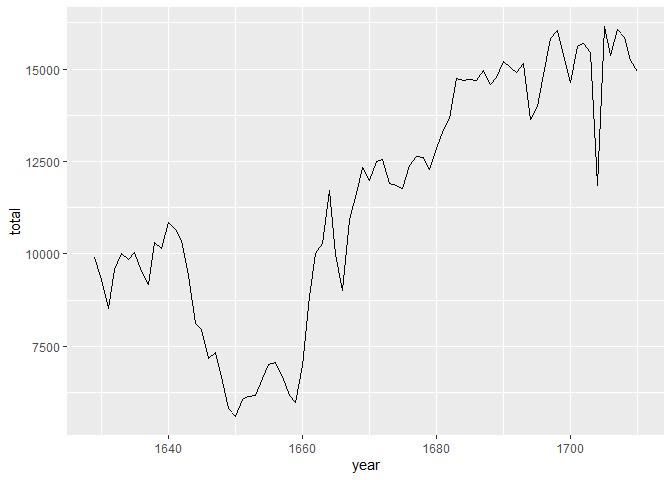
\includegraphics{lab_1_files/figure-latex/plot-total-vs-year-line-1.pdf}

Note that using \texttt{geom\_line()} instead of \texttt{geom\_point()}
results in a line plot instead of a scatter plot. You want both? Just
layer them on:

\begin{Shaded}
\begin{Highlighting}[]
\FunctionTok{ggplot}\NormalTok{(}\AttributeTok{data =}\NormalTok{ arbuthnot, }\FunctionTok{aes}\NormalTok{(}\AttributeTok{x =}\NormalTok{ year, }\AttributeTok{y =}\NormalTok{ total)) }\SpecialCharTok{+}
  \FunctionTok{geom\_line}\NormalTok{() }\SpecialCharTok{+}
  \FunctionTok{geom\_point}\NormalTok{()}
\end{Highlighting}
\end{Shaded}

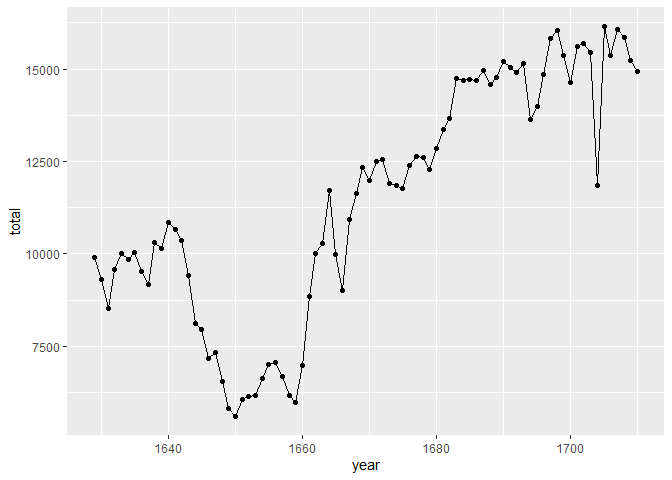
\includegraphics{lab_1_files/figure-latex/plot-total-vs-year-line-and-point-1.pdf}

\phantomsection\label{exercise}
\textbf{Exercise}: Now, generate a plot of the proportion of boys born
over time. What do you see?

\begin{Shaded}
\begin{Highlighting}[]
\CommentTok{\# type your code for the Exercise here, and Knit}
\FunctionTok{ggplot}\NormalTok{(}\AttributeTok{data =}\NormalTok{ arbuthnot, }\FunctionTok{aes}\NormalTok{(}\AttributeTok{x =}\NormalTok{ year, }\AttributeTok{y =}\NormalTok{ boys)) }\SpecialCharTok{+}
  \FunctionTok{geom\_line}\NormalTok{() }\SpecialCharTok{+}
  \FunctionTok{geom\_point}\NormalTok{()}
\end{Highlighting}
\end{Shaded}

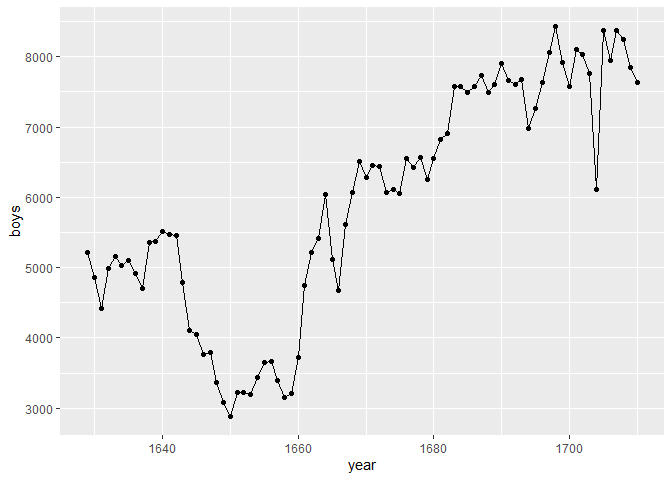
\includegraphics{lab_1_files/figure-latex/plot-proportion-of-boys-over-time-1.pdf}

Finally, in addition to simple mathematical operators like subtraction
and division, you can ask R to make comparisons like greater than,
\texttt{\textgreater{}}, less than, \texttt{\textless{}}, and equality,
\texttt{==}. For example, we can ask if boys outnumber girls in each
year with the expression

\begin{Shaded}
\begin{Highlighting}[]
\NormalTok{arbuthnot }\OtherTok{\textless{}{-}}\NormalTok{ arbuthnot }\SpecialCharTok{\%\textgreater{}\%}
  \FunctionTok{mutate}\NormalTok{(}\AttributeTok{more\_boys =}\NormalTok{ boys }\SpecialCharTok{\textgreater{}}\NormalTok{ girls)}
\end{Highlighting}
\end{Shaded}

This command add a new variable to the \texttt{arbuthnot} data frame
containing the values of either \texttt{TRUE} if that year had more boys
than girls, or \texttt{FALSE} if that year did not (the answer may
surprise you). This variable contains different kind of data than we
have considered so far. All other columns in the \texttt{arbuthnot} data
frame have values are numerical (the year, the number of boys and
girls). Here, we've asked R to create \emph{logical} data, data where
the values are either \texttt{TRUE} or \texttt{FALSE}. In general, data
analysis will involve many different kinds of data types, and one reason
for using R is that it is able to represent and compute with many of
them.

\subsection{Dataset 2: Present birth
records}\label{dataset-2-present-birth-records}

In the previous few pages, you recreated some of the displays and
preliminary analysis of Arbuthnot's baptism data. Next you will do a
similar analysis, but for present day birth records in the United
States. Load up the present day data with the following command.

\begin{Shaded}
\begin{Highlighting}[]
\FunctionTok{data}\NormalTok{(present)}
\end{Highlighting}
\end{Shaded}

The data are stored in a data frame called \texttt{present} which should
now be loaded in your workspace.

\begin{enumerate}
\def\labelenumi{\arabic{enumi}.}
\setcounter{enumi}{3}
\tightlist
\item
  How many variables are included in this data set?

  2

  3

  4

  74

  2013
\end{enumerate}

\begin{Shaded}
\begin{Highlighting}[]
\CommentTok{\# type your code for Question 4 here, and Knit}
\NormalTok{present}
\end{Highlighting}
\end{Shaded}

\begin{verbatim}
## # A tibble: 74 x 3
##     year    boys   girls
##    <dbl>   <dbl>   <dbl>
##  1  1940 1211684 1148715
##  2  1941 1289734 1223693
##  3  1942 1444365 1364631
##  4  1943 1508959 1427901
##  5  1944 1435301 1359499
##  6  1945 1404587 1330869
##  7  1946 1691220 1597452
##  8  1947 1899876 1800064
##  9  1948 1813852 1721216
## 10  1949 1826352 1733177
## # i 64 more rows
\end{verbatim}

\phantomsection\label{exercise}
\textbf{Exercise}: What years are included in this dataset?
\textbf{Hint:} Use the \texttt{range} function and
\texttt{present\$year} as its argument.

\begin{Shaded}
\begin{Highlighting}[]
\CommentTok{\# type your code for Exercise here, and Knit}
\FunctionTok{range}\NormalTok{(present}\SpecialCharTok{$}\NormalTok{year)}
\end{Highlighting}
\end{Shaded}

\begin{verbatim}
## [1] 1940 2013
\end{verbatim}

\begin{enumerate}
\def\labelenumi{\arabic{enumi}.}
\setcounter{enumi}{4}
\tightlist
\item
  Calculate the total number of births for each year and store these
  values in a new variable called \texttt{total} in the \texttt{present}
  dataset. Then, calculate the proportion of boys born each year and
  store these values in a new variable called \texttt{prop\_boys} in the
  same dataset. Plot these values over time and based on the plot
  determine if the following statement is true or false: The proportion
  of boys born in the US has decreased over time.

  True

  False
\end{enumerate}

\begin{Shaded}
\begin{Highlighting}[]
\CommentTok{\# type your code for Question 5 here, and Knit}
\NormalTok{present}\SpecialCharTok{$}\NormalTok{total }\OtherTok{=}\NormalTok{ present}\SpecialCharTok{$}\NormalTok{boys }\SpecialCharTok{+}\NormalTok{ present}\SpecialCharTok{$}\NormalTok{girls}
\NormalTok{present}\SpecialCharTok{$}\NormalTok{prop\_boys }\OtherTok{=}\NormalTok{ present}\SpecialCharTok{$}\NormalTok{boys }\SpecialCharTok{/}\NormalTok{ present}\SpecialCharTok{$}\NormalTok{total}
\end{Highlighting}
\end{Shaded}

\begin{Shaded}
\begin{Highlighting}[]
\FunctionTok{plot}\NormalTok{(present}\SpecialCharTok{$}\NormalTok{year, present}\SpecialCharTok{$}\NormalTok{prop\_boys)}
\end{Highlighting}
\end{Shaded}

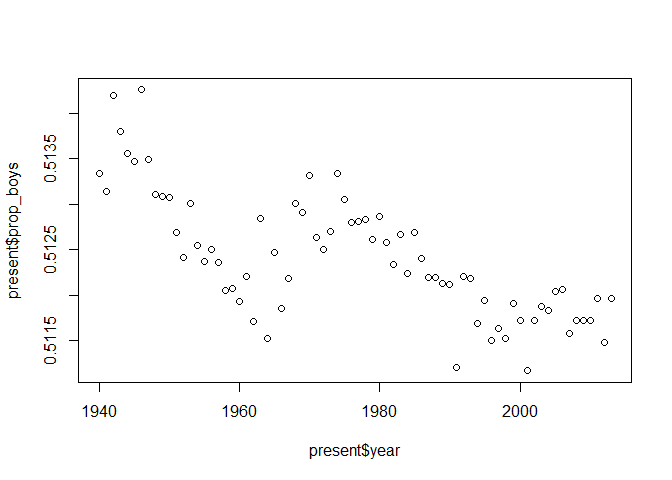
\includegraphics{lab_1_files/figure-latex/unnamed-chunk-1-1.pdf}

\begin{enumerate}
\def\labelenumi{\arabic{enumi}.}
\setcounter{enumi}{5}
\tightlist
\item
  Create a new variable called \texttt{more\_boys} which contains the
  value of either \texttt{TRUE} if that year had more boys than girls,
  or \texttt{FALSE} if that year did not. Based on this variable which
  of the following statements is true?

  Every year there are more girls born than boys.

  Every year there are more boys born than girls.

  Half of the years there are more boys born, and the other half more
  girls born.
\end{enumerate}

\begin{Shaded}
\begin{Highlighting}[]
\CommentTok{\# type your code for Question 6 here, and Knit}
\NormalTok{present}\SpecialCharTok{$}\NormalTok{more\_boys }\OtherTok{=}\NormalTok{ present}\SpecialCharTok{$}\NormalTok{boys }\SpecialCharTok{\textgreater{}}\NormalTok{ present}\SpecialCharTok{$}\NormalTok{girls}
\FunctionTok{plot}\NormalTok{(present}\SpecialCharTok{$}\NormalTok{year, present}\SpecialCharTok{$}\NormalTok{more\_boys)}
\end{Highlighting}
\end{Shaded}

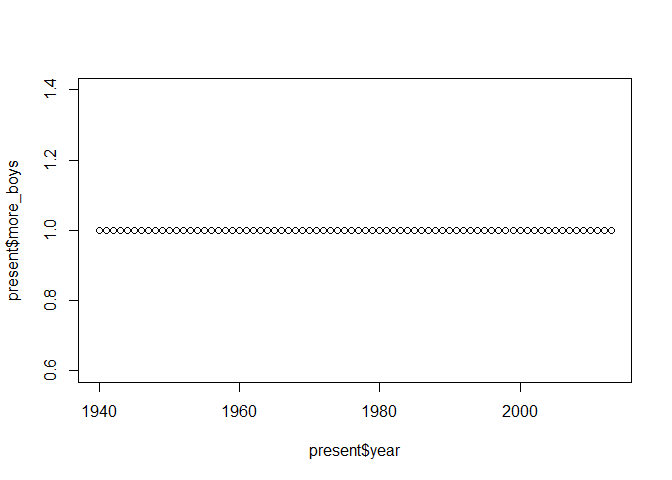
\includegraphics{lab_1_files/figure-latex/more-boys-per-year-1.pdf}

\begin{enumerate}
\def\labelenumi{\arabic{enumi}.}
\setcounter{enumi}{6}
\tightlist
\item
  Calculate the boy-to-girl ratio each year, and store these values in a
  new variable called \texttt{prop\_boy\_girl} in the \texttt{present}
  dataset. Plot these values over time. Which of the following best
  describes the trend?

  There appears to be no trend in the boy-to-girl ratio from 1940 to
  2013.

  There is initially an increase in boy-to-girl ratio, which peaks
  around 1960. After 1960 there is a decrease in the boy-to-girl ratio,
  but the number begins to increase in the mid 1970s.

  There is initially a decrease in the boy-to-girl ratio, and then an
  increase between 1960 and 1970, followed by a decrease.

  The boy-to-girl ratio has increased over time.

  There is an initial decrease in the boy-to-girl ratio born but this
  number appears to level around 1960 and remain constant since then.
\end{enumerate}

\begin{Shaded}
\begin{Highlighting}[]
\CommentTok{\# type your code for Question 7 here, and Knit}
\NormalTok{present}\SpecialCharTok{$}\NormalTok{prop\_boy\_girl }\OtherTok{=}\NormalTok{ present}\SpecialCharTok{$}\NormalTok{boys }\SpecialCharTok{/}\NormalTok{ present}\SpecialCharTok{$}\NormalTok{girls}
\FunctionTok{plot}\NormalTok{(present}\SpecialCharTok{$}\NormalTok{year, present}\SpecialCharTok{$}\NormalTok{prop\_boy\_girl)}
\end{Highlighting}
\end{Shaded}

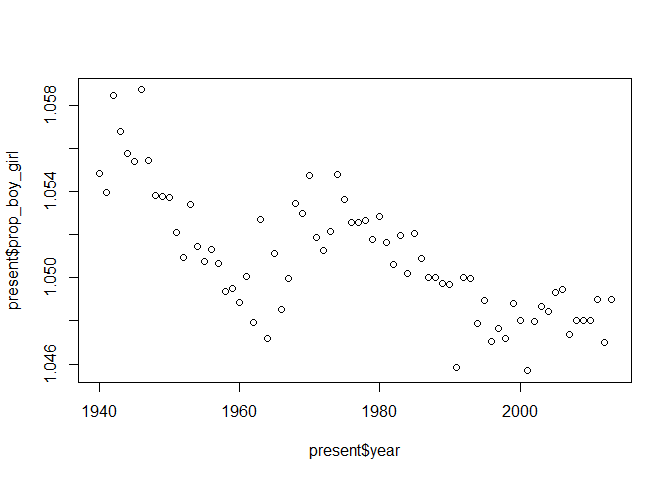
\includegraphics{lab_1_files/figure-latex/prop-boy-girl-over-time-1.pdf}

\begin{enumerate}
\def\labelenumi{\arabic{enumi}.}
\setcounter{enumi}{7}
\tightlist
\item
  In what year did we see the most total number of births in the U.S.?
  \emph{Hint:} Sort your dataset in descending order based on the
  \texttt{total} column. You can do this interactively in the data
  viewer by clicking on the arrows next to the variable names. Or to
  arrange the data in a descenting order with new function:
  \texttt{descr} (for descending order).

  1940

  1957

  1961

  1991

  2007
\end{enumerate}

\begin{Shaded}
\begin{Highlighting}[]
\CommentTok{\# type your code for Question 8 here}
\CommentTok{\# sample code is provided below, edit as necessary, uncomment, and then Knit}
\NormalTok{present }\SpecialCharTok{\%\textgreater{}\%}
  \FunctionTok{mutate}\NormalTok{(}\AttributeTok{total =}\NormalTok{ present}\SpecialCharTok{$}\NormalTok{boys }\SpecialCharTok{+}\NormalTok{ present}\SpecialCharTok{$}\NormalTok{girls) }\SpecialCharTok{\%\textgreater{}\%}
  \FunctionTok{arrange}\NormalTok{(}\FunctionTok{desc}\NormalTok{(total))}
\end{Highlighting}
\end{Shaded}

\begin{verbatim}
## # A tibble: 74 x 7
##     year    boys   girls   total prop_boys more_boys prop_boy_girl
##    <dbl>   <dbl>   <dbl>   <dbl>     <dbl> <lgl>             <dbl>
##  1  2007 2208071 2108162 4316233     0.512 TRUE               1.05
##  2  1961 2186274 2082052 4268326     0.512 TRUE               1.05
##  3  2006 2184237 2081318 4265555     0.512 TRUE               1.05
##  4  1960 2179708 2078142 4257850     0.512 TRUE               1.05
##  5  1957 2179960 2074824 4254784     0.512 TRUE               1.05
##  6  2008 2173625 2074069 4247694     0.512 TRUE               1.05
##  7  1959 2173638 2071158 4244796     0.512 TRUE               1.05
##  8  1958 2152546 2051266 4203812     0.512 TRUE               1.05
##  9  1962 2132466 2034896 4167362     0.512 TRUE               1.05
## 10  1956 2133588 2029502 4163090     0.513 TRUE               1.05
## # i 64 more rows
\end{verbatim}

\subsection{Resources for learning R and working in
RStudio}\label{resources-for-learning-r-and-working-in-rstudio}

That was a short introduction to R and RStudio, but we will provide you
with more functions and a more complete sense of the language as the
course progresses. You might find the following tips and resources
helpful.

\begin{itemize}
\item
  In this course we will be using the \texttt{dplyr} (for data
  wrangling) and \texttt{ggplot2} (for data visualization) extensively.
  If you are googling for R code, make sure to also include these
  package names in your search query. For example, instead of googling
  ``scatterplot in R'', google ``scatterplot in R with ggplot2''.
\item
  The following cheathseets may come in handy throughout the course.
  Note that some of the code on these cheatsheets may be too advanced
  for this course, however majority of it will become useful as you
  progress through the course material.

  \begin{itemize}
  \tightlist
  \item
    \href{http://www.rstudio.com/wp-content/uploads/2015/02/data-wrangling-cheatsheet.pdf}{Data
    wrangling cheatsheet}
  \item
    \href{http://www.rstudio.com/wp-content/uploads/2015/12/ggplot2-cheatsheet-2.0.pdf}{Data
    visualization cheatsheet}
  \item
    \href{http://www.rstudio.com/wp-content/uploads/2016/03/rmarkdown-cheatsheet-2.0.pdf}{R
    Markdown}
  \end{itemize}
\item
  While you will get plenty of exercise working with these packages in
  the labs of this course, if you would like further opportunities to
  practice we recommend checking out the relevant courses at
  \href{https://www.datacamp.com/courses}{DataCamp}.
\end{itemize}

\phantomsection\label{license}
This is a derivative of an
\href{https://www.openintro.org/stat/labs.php}{OpenIntro} lab, and is
released under a
\href{https://creativecommons.org/licenses/by-nc-sa/3.0/us/}{Attribution-NonCommercial-ShareAlike
3.0 United States} license.

\end{document}
